% Options for packages loaded elsewhere
\PassOptionsToPackage{unicode}{hyperref}
\PassOptionsToPackage{hyphens}{url}
%
\documentclass[
  12pt,
]{article}
\usepackage{amsmath,amssymb}
\usepackage{iftex}
\ifPDFTeX
  \usepackage[T1]{fontenc}
  \usepackage[utf8]{inputenc}
  \usepackage{textcomp} % provide euro and other symbols
\else % if luatex or xetex
  \usepackage{unicode-math} % this also loads fontspec
  \defaultfontfeatures{Scale=MatchLowercase}
  \defaultfontfeatures[\rmfamily]{Ligatures=TeX,Scale=1}
\fi
\usepackage{lmodern}
\ifPDFTeX\else
  % xetex/luatex font selection
\fi
% Use upquote if available, for straight quotes in verbatim environments
\IfFileExists{upquote.sty}{\usepackage{upquote}}{}
\IfFileExists{microtype.sty}{% use microtype if available
  \usepackage[]{microtype}
  \UseMicrotypeSet[protrusion]{basicmath} % disable protrusion for tt fonts
}{}
\makeatletter
\@ifundefined{KOMAClassName}{% if non-KOMA class
  \IfFileExists{parskip.sty}{%
    \usepackage{parskip}
  }{% else
    \setlength{\parindent}{0pt}
    \setlength{\parskip}{6pt plus 2pt minus 1pt}}
}{% if KOMA class
  \KOMAoptions{parskip=half}}
\makeatother
\usepackage{xcolor}
\usepackage[left=1.5cm,right=1.5cm,top=1cm,bottom=1.5cm]{geometry}
\usepackage{color}
\usepackage{fancyvrb}
\newcommand{\VerbBar}{|}
\newcommand{\VERB}{\Verb[commandchars=\\\{\}]}
\DefineVerbatimEnvironment{Highlighting}{Verbatim}{commandchars=\\\{\}}
% Add ',fontsize=\small' for more characters per line
\usepackage{framed}
\definecolor{shadecolor}{RGB}{248,248,248}
\newenvironment{Shaded}{\begin{snugshade}}{\end{snugshade}}
\newcommand{\AlertTok}[1]{\textcolor[rgb]{0.94,0.16,0.16}{#1}}
\newcommand{\AnnotationTok}[1]{\textcolor[rgb]{0.56,0.35,0.01}{\textbf{\textit{#1}}}}
\newcommand{\AttributeTok}[1]{\textcolor[rgb]{0.13,0.29,0.53}{#1}}
\newcommand{\BaseNTok}[1]{\textcolor[rgb]{0.00,0.00,0.81}{#1}}
\newcommand{\BuiltInTok}[1]{#1}
\newcommand{\CharTok}[1]{\textcolor[rgb]{0.31,0.60,0.02}{#1}}
\newcommand{\CommentTok}[1]{\textcolor[rgb]{0.56,0.35,0.01}{\textit{#1}}}
\newcommand{\CommentVarTok}[1]{\textcolor[rgb]{0.56,0.35,0.01}{\textbf{\textit{#1}}}}
\newcommand{\ConstantTok}[1]{\textcolor[rgb]{0.56,0.35,0.01}{#1}}
\newcommand{\ControlFlowTok}[1]{\textcolor[rgb]{0.13,0.29,0.53}{\textbf{#1}}}
\newcommand{\DataTypeTok}[1]{\textcolor[rgb]{0.13,0.29,0.53}{#1}}
\newcommand{\DecValTok}[1]{\textcolor[rgb]{0.00,0.00,0.81}{#1}}
\newcommand{\DocumentationTok}[1]{\textcolor[rgb]{0.56,0.35,0.01}{\textbf{\textit{#1}}}}
\newcommand{\ErrorTok}[1]{\textcolor[rgb]{0.64,0.00,0.00}{\textbf{#1}}}
\newcommand{\ExtensionTok}[1]{#1}
\newcommand{\FloatTok}[1]{\textcolor[rgb]{0.00,0.00,0.81}{#1}}
\newcommand{\FunctionTok}[1]{\textcolor[rgb]{0.13,0.29,0.53}{\textbf{#1}}}
\newcommand{\ImportTok}[1]{#1}
\newcommand{\InformationTok}[1]{\textcolor[rgb]{0.56,0.35,0.01}{\textbf{\textit{#1}}}}
\newcommand{\KeywordTok}[1]{\textcolor[rgb]{0.13,0.29,0.53}{\textbf{#1}}}
\newcommand{\NormalTok}[1]{#1}
\newcommand{\OperatorTok}[1]{\textcolor[rgb]{0.81,0.36,0.00}{\textbf{#1}}}
\newcommand{\OtherTok}[1]{\textcolor[rgb]{0.56,0.35,0.01}{#1}}
\newcommand{\PreprocessorTok}[1]{\textcolor[rgb]{0.56,0.35,0.01}{\textit{#1}}}
\newcommand{\RegionMarkerTok}[1]{#1}
\newcommand{\SpecialCharTok}[1]{\textcolor[rgb]{0.81,0.36,0.00}{\textbf{#1}}}
\newcommand{\SpecialStringTok}[1]{\textcolor[rgb]{0.31,0.60,0.02}{#1}}
\newcommand{\StringTok}[1]{\textcolor[rgb]{0.31,0.60,0.02}{#1}}
\newcommand{\VariableTok}[1]{\textcolor[rgb]{0.00,0.00,0.00}{#1}}
\newcommand{\VerbatimStringTok}[1]{\textcolor[rgb]{0.31,0.60,0.02}{#1}}
\newcommand{\WarningTok}[1]{\textcolor[rgb]{0.56,0.35,0.01}{\textbf{\textit{#1}}}}
\usepackage{graphicx}
\makeatletter
\def\maxwidth{\ifdim\Gin@nat@width>\linewidth\linewidth\else\Gin@nat@width\fi}
\def\maxheight{\ifdim\Gin@nat@height>\textheight\textheight\else\Gin@nat@height\fi}
\makeatother
% Scale images if necessary, so that they will not overflow the page
% margins by default, and it is still possible to overwrite the defaults
% using explicit options in \includegraphics[width, height, ...]{}
\setkeys{Gin}{width=\maxwidth,height=\maxheight,keepaspectratio}
% Set default figure placement to htbp
\makeatletter
\def\fps@figure{htbp}
\makeatother
\setlength{\emergencystretch}{3em} % prevent overfull lines
\providecommand{\tightlist}{%
  \setlength{\itemsep}{0pt}\setlength{\parskip}{0pt}}
\setcounter{secnumdepth}{-\maxdimen} % remove section numbering
\ifLuaTeX
  \usepackage{selnolig}  % disable illegal ligatures
\fi
\IfFileExists{bookmark.sty}{\usepackage{bookmark}}{\usepackage{hyperref}}
\IfFileExists{xurl.sty}{\usepackage{xurl}}{} % add URL line breaks if available
\urlstyle{same}
\hypersetup{
  pdftitle={Prediction of inflation rate with times-series data},
  pdfauthor={Guojun Ma},
  hidelinks,
  pdfcreator={LaTeX via pandoc}}

\title{Prediction of inflation rate with times-series data}
\author{Guojun Ma}
\date{oday}

\begin{document}
\maketitle

{
\setcounter{tocdepth}{3}
\tableofcontents
}
\hypertarget{section-1---introduction}{%
\subsection{Section 1 - Introduction}\label{section-1---introduction}}

The goal of this project is to build a statistical model to forecast the
interest rate of Canada. By analyzing the historical economic and
financial data from the website of international monetary policy(IMF),
we would like to discover the underlying mathematical law of inflation.
Economic indicators for measuring the inflation rate included the
Consumer price index (CPI), the producer price index(PPI) and the GDP
deflator. The most commonly used one is CPI, which is defined as the
price of one fixed basket of consumer goods and services in one period.
CPI include the cost of food, beverages, housing, education,
transportation and medical care. The unit of CPI s measured in
percentage, which is compared to the based year. For example, if the
base year is \(2010\), then the CPI of \(125\) means that the price
increased by \(125\) percent compared to the year \(2010\).

There are many statistical models to predict inflation rates in the
existing literature. For example, the Phillips curve shows the inverse
trade-off between rates of inflation and rates of unemployment
\cite{bib1}. One other method involves regressions based on implicit
expectations derived from asset prices, such as nominal Treasury debt
\cite{bib2, bib3}. In this project, we adopt the method that prediction
based only on past inflation rate. This leads to time series models such
as auto-regressive integrated moving average (ARIMA) models.

We also examine the correlation and causal relation of inflation and its
predictors such as government spending. Economists believe that the
causes of inflation included increased government spending,
demand/supply shocks and unemployment rate. We would like to investigate
how strongly these variables are correlated. By examining the
correlation of time lag variable, it is possible to find causal
relations. We also analyze the US data and examine the cross-correlation
with the Canadian data.

\hypertarget{section-2---analysis-of-the-time-series-data}{%
\subsection{Section 2 - Analysis of the time series
data}\label{section-2---analysis-of-the-time-series-data}}

The figure belows shows the CPI for the last ten years, where the unit
is in the month.

\begin{Shaded}
\begin{Highlighting}[]
\FunctionTok{plot}\NormalTok{(CPI, }\AttributeTok{main =} \StringTok{"Inflation rate of Canada  "}\NormalTok{, }\AttributeTok{xlab =} \StringTok{"Year(based year = 2010)"}\NormalTok{, }\AttributeTok{ylab =} \StringTok{"CPI"}\NormalTok{)}
\end{Highlighting}
\end{Shaded}

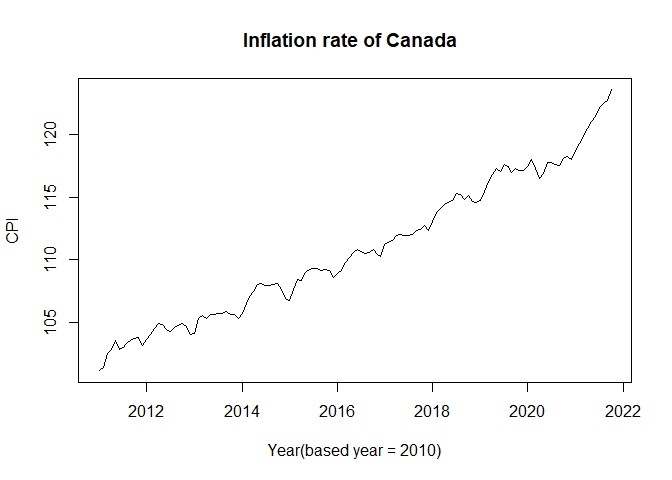
\includegraphics{analysis-of-inflation-using-ARIMA-modelling_files/figure-latex/unnamed-chunk-2-1.pdf}

The figure shows an upward trend, and the rate of increase is the
fastest over the years \(2020\) and \(2021\) because of the pandemic. We
apply the difference operator to the data and graph the new data in
figure. We can see that the new time series is weakly stationary.

\begin{Shaded}
\begin{Highlighting}[]
\NormalTok{stat\_CPI }\OtherTok{=} \FunctionTok{diff}\NormalTok{(CPI)}
\FunctionTok{plot}\NormalTok{(stat\_CPI, }\AttributeTok{main =} \StringTok{"First difference"}\NormalTok{, }\AttributeTok{xlab =} \StringTok{"Year"}\NormalTok{, }\AttributeTok{ylab =} \StringTok{"CPI"}\NormalTok{)}
\end{Highlighting}
\end{Shaded}

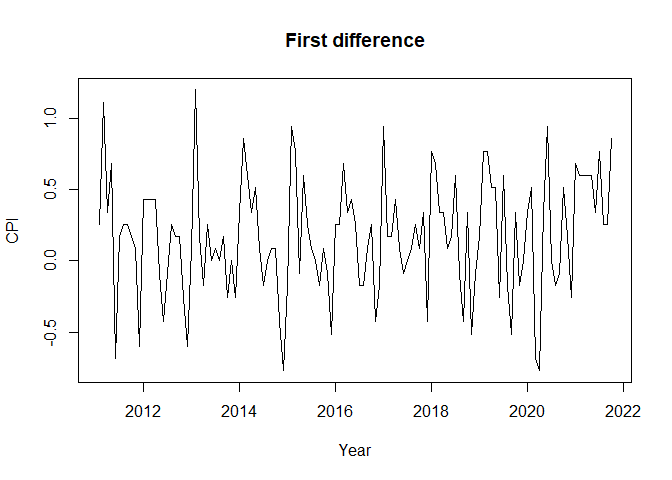
\includegraphics{analysis-of-inflation-using-ARIMA-modelling_files/figure-latex/unnamed-chunk-3-1.pdf}

\hypertarget{section-3---diagotistic-of-the-model}{%
\subsection{Section 3 - Diagotistic of the
model}\label{section-3---diagotistic-of-the-model}}

The plots of ACF and PACF are shown in the figure below:

\begin{Shaded}
\begin{Highlighting}[]
\FunctionTok{acf2}\NormalTok{(stat\_CPI, }\DecValTok{50}\NormalTok{, }\AttributeTok{main =} \StringTok{""}\NormalTok{)}
\end{Highlighting}
\end{Shaded}

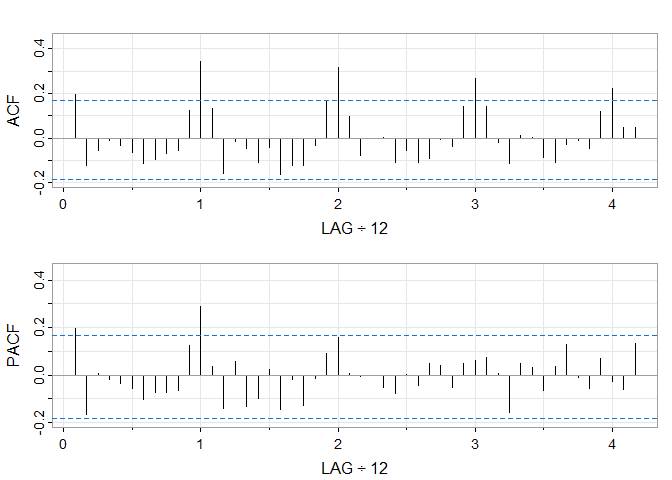
\includegraphics{analysis-of-inflation-using-ARIMA-modelling_files/figure-latex/unnamed-chunk-4-1.pdf}

\begin{verbatim}
##      [,1]  [,2]  [,3]  [,4]  [,5]  [,6]  [,7]  [,8]  [,9] [,10] [,11] [,12]
## ACF   0.2 -0.12 -0.05 -0.01 -0.03 -0.06 -0.11 -0.10 -0.07 -0.06  0.12  0.34
## PACF  0.2 -0.16  0.01 -0.02 -0.04 -0.06 -0.10 -0.07 -0.07 -0.07  0.13  0.29
##      [,13] [,14] [,15] [,16] [,17] [,18] [,19] [,20] [,21] [,22] [,23] [,24]
## ACF   0.13 -0.16 -0.01 -0.05 -0.11 -0.04 -0.16 -0.12 -0.12 -0.03  0.17  0.32
## PACF  0.04 -0.14  0.06 -0.13 -0.10  0.02 -0.14 -0.02 -0.13 -0.02  0.09  0.16
##      [,25] [,26] [,27] [,28] [,29] [,30] [,31] [,32] [,33] [,34] [,35] [,36]
## ACF   0.10 -0.08     0  0.01 -0.11 -0.06 -0.11 -0.09  0.00 -0.04  0.14  0.27
## PACF  0.01  0.00     0 -0.05 -0.08  0.00 -0.04  0.05  0.04 -0.05  0.05  0.06
##      [,37] [,38] [,39] [,40] [,41] [,42] [,43] [,44] [,45] [,46] [,47] [,48]
## ACF   0.14 -0.02 -0.11  0.01  0.00 -0.09 -0.11 -0.03 -0.01 -0.05  0.12  0.22
## PACF  0.07  0.01 -0.16  0.05  0.03 -0.07  0.04  0.13 -0.01 -0.06  0.07 -0.03
##      [,49] [,50]
## ACF   0.05  0.05
## PACF -0.06  0.13
\end{verbatim}

The ACF plot shows the presence of seasonal correlation where the season
is equal to \(12\) months. The PACF shows the seasonal correlation cuts
off after 2 seasons. This suggests we fit the model with parameters
\(P = 2, Q = 0\) and \(s = 12\). By observing the figure at the smaller
lag, both the ACF and PACF are tailing off. So we try to fit the
non-seasonal component with \(p = 1\) and \(q = 1\). The model we get
for the original time series \(x_t\) is

\begin{equation}
    \label{SARIMA model}
    ( 1 - \Phi_1 B^{12} - \Phi_2  B^{24} )( 1 - \phi_1 B) \triangledown x_t = \delta + ( 1 + \theta_1 B) w_t
\end{equation} Where \(\Phi, \phi, \theta, \delta\) are the coefficients
of the model.

Compare to the other coefficients in the model, the standard error for
\(\theta_1, \phi_1\) are quiet large. Fortunately, the P values for
these coefficients are large. By eliminating these two we get a
simplified model. We fit the model \begin{equation}
    \label{SARIMA2}
    ( 1 - \Phi_1 B^{12} - \Phi_2  B^{24} ) \triangledown x_t = \delta + w_t
\end{equation}

\begin{Shaded}
\begin{Highlighting}[]
\NormalTok{fitted\_model }\OtherTok{=} \FunctionTok{sarima}\NormalTok{(CPI, }\DecValTok{0}\NormalTok{, }\DecValTok{1}\NormalTok{, }\DecValTok{0}\NormalTok{, }\DecValTok{2}\NormalTok{, }\DecValTok{0}\NormalTok{, }\DecValTok{0}\NormalTok{, }\DecValTok{12}\NormalTok{)}
\end{Highlighting}
\end{Shaded}

\begin{verbatim}
## initial  value -0.910514 
## iter   2 value -1.002753
## iter   3 value -1.022059
## iter   4 value -1.022995
## iter   5 value -1.023603
## iter   6 value -1.023862
## iter   7 value -1.023898
## iter   8 value -1.023902
## iter   9 value -1.023902
## iter  10 value -1.023902
## iter  10 value -1.023902
## iter  10 value -1.023902
## final  value -1.023902 
## converged
## initial  value -1.010296 
## iter   2 value -1.012201
## iter   3 value -1.013097
## iter   4 value -1.013162
## iter   5 value -1.013207
## iter   6 value -1.013212
## iter   7 value -1.013213
## iter   7 value -1.013213
## iter   7 value -1.013213
## final  value -1.013213 
## converged
## <><><><><><><><><><><><><><>
##  
## Coefficients: 
##          Estimate     SE t.value p.value
## sar1       0.2692 0.0882  3.0522  0.0028
## sar2       0.3015 0.0966  3.1200  0.0022
## constant   0.1909 0.0627  3.0463  0.0028
## 
## sigma^2 estimated as 0.1275677 on 126 degrees of freedom 
##  
## AIC = 0.8734669  AICc = 0.8749553  BIC = 0.9621433 
## 
\end{verbatim}

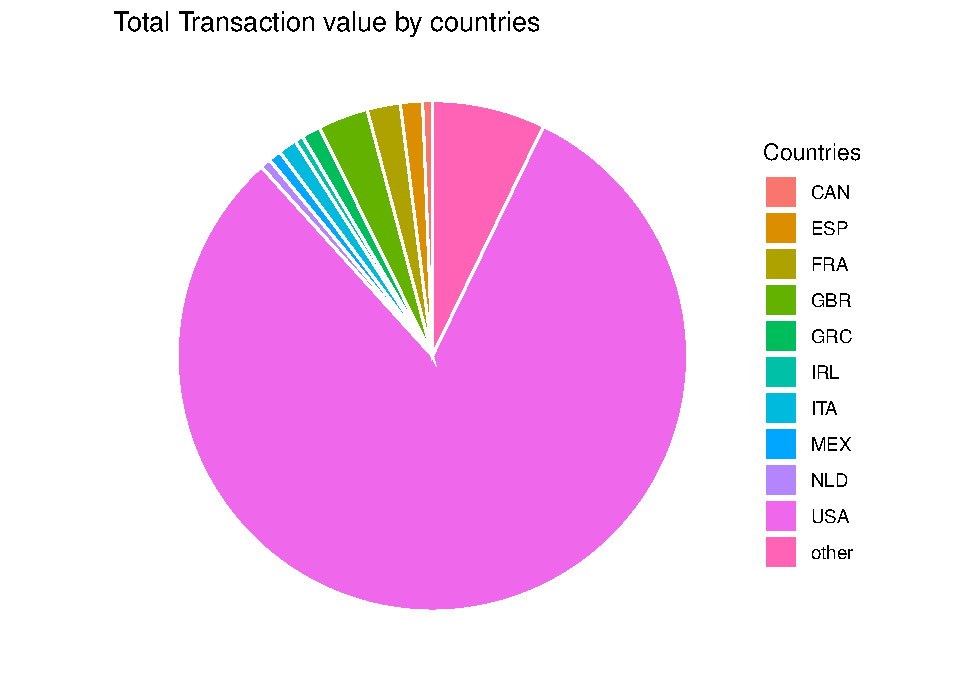
\includegraphics{analysis-of-inflation-using-ARIMA-modelling_files/figure-latex/unnamed-chunk-5-1.pdf}

\begin{Shaded}
\begin{Highlighting}[]
\FunctionTok{sarima.for}\NormalTok{(CPI, }\DecValTok{12}\NormalTok{, }\DecValTok{0}\NormalTok{, }\DecValTok{1}\NormalTok{, }\DecValTok{0}\NormalTok{, }\DecValTok{2}\NormalTok{, }\DecValTok{0}\NormalTok{, }\DecValTok{0}\NormalTok{ , }\DecValTok{12}\NormalTok{ )}
\end{Highlighting}
\end{Shaded}

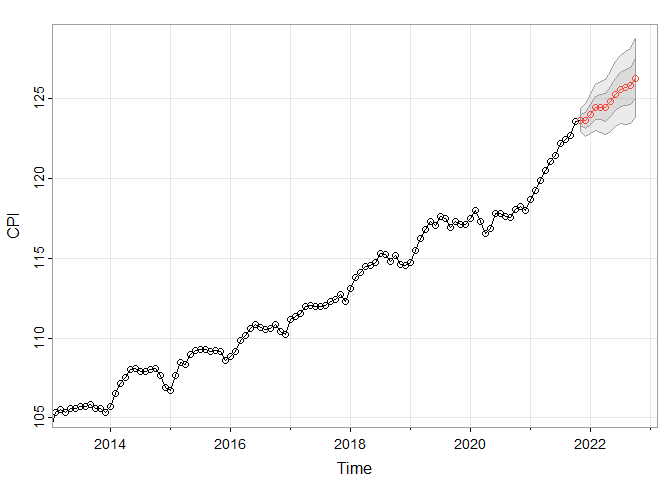
\includegraphics{analysis-of-inflation-using-ARIMA-modelling_files/figure-latex/unnamed-chunk-5-2.pdf}

\begin{verbatim}
## $pred
##           Jan      Feb      Mar      Apr      May      Jun      Jul      Aug
## 2021                                                                        
## 2022 124.0141 124.4131 124.4497 124.4604 124.8077 125.2669 125.5568 125.6563
##           Sep      Oct      Nov      Dec
## 2021                   123.6311 123.6437
## 2022 125.7817 126.2501                  
## 
## $se
##            Jan       Feb       Mar       Apr       May       Jun       Jul
## 2021                                                                      
## 2022 0.6186300 0.7143324 0.7986479 0.8748750 0.9449730 1.0102186 1.0714986
##            Aug       Sep       Oct       Nov       Dec
## 2021                               0.3571662 0.5051093
## 2022 1.1294587 1.1845863 1.2372600
\end{verbatim}

\pagebreak
\begin{thebibliography}{}
    \bibitem{bib1}
    Atkeson Andrew, and Lee E.Ohanian
    \textit{Are Phillip Curves Useful For Forecasting Inflation?}
    Federal Reserve Bank of Minneapolis Quarterly review
    25(1) : 2 - 11
    Available at  http://www.minneapolisfed.org/research/QR/QR2511.pdf 
    
    \bibitem{bib2}
    Mishkin, Frederic S.
    \textit{What Does the Term Structure Tell us about Future inflation?}
    Journal of Monetary Economics 
    25(1) : 77 - 95
    
    \bibitem{bib3}
    Mishkin, Frederic S.
    \textit{The Information in the Longer-Maturity Term Structure about future inflation.}
    Quarterly Journal of Economics 
    105(3) : 815 - 828

\end{thebibliography}

\end{document}
